\chapter{SIMULACIONES CON DISTINTOS COEFICIENTES DE DILATACIÓN ADIABÁTICA}
\label{cap:5}
En este último capítulo se comparan los resultados obtenidos en simulaciones del mismo problema de condición inicial pero con distinto coeficiente de dilatación adiabática $\gamma$, con el fin de obtener una intuición física, a través de la simulación, de cómo varía el comportamiento de un gas cuando el número de grados de libertad interno del mismo cambia.
\section{Consideraciones preliminares}
Dado que el coeficiente de dilatación adiabática está relacionado explícitamente con el número de grados de libertad interno de un gas $\alpha$,
\begin{equation}
	\gamma = \frac{\alpha + 2}{\alpha},
\end{equation}
es conveniente definir distintos valores para $\gamma$ que dependan de un valor razonable para $\alpha$.

En las anteriores simulaciones, se calculó $\gamma$ para un gas diatómico como el aire. La justificación del número de grados de libertad de estos gases se dio en la sección \ref{sec:ecuacion-de-estado-gas}. En este caso:
\begin{equation}
	\alpha = 5 \implies \gamma = 7/5 = 1.4.
\end{equation}
Entonces, se considerarán experimentos de gases con 16 y 32 grados de libertad internos, que corresponden a $\gamma=1.125$ y $\gamma=1.0625$ respectivamente.
\section{Test de Sod}
El problema de condiciones iniciales que se estudiará con simulaciones con distintos valores para $\gamma$ es el test de Sod (sección \ref{sec:sod_con_entropy148}).
\begin{figure}[H]
	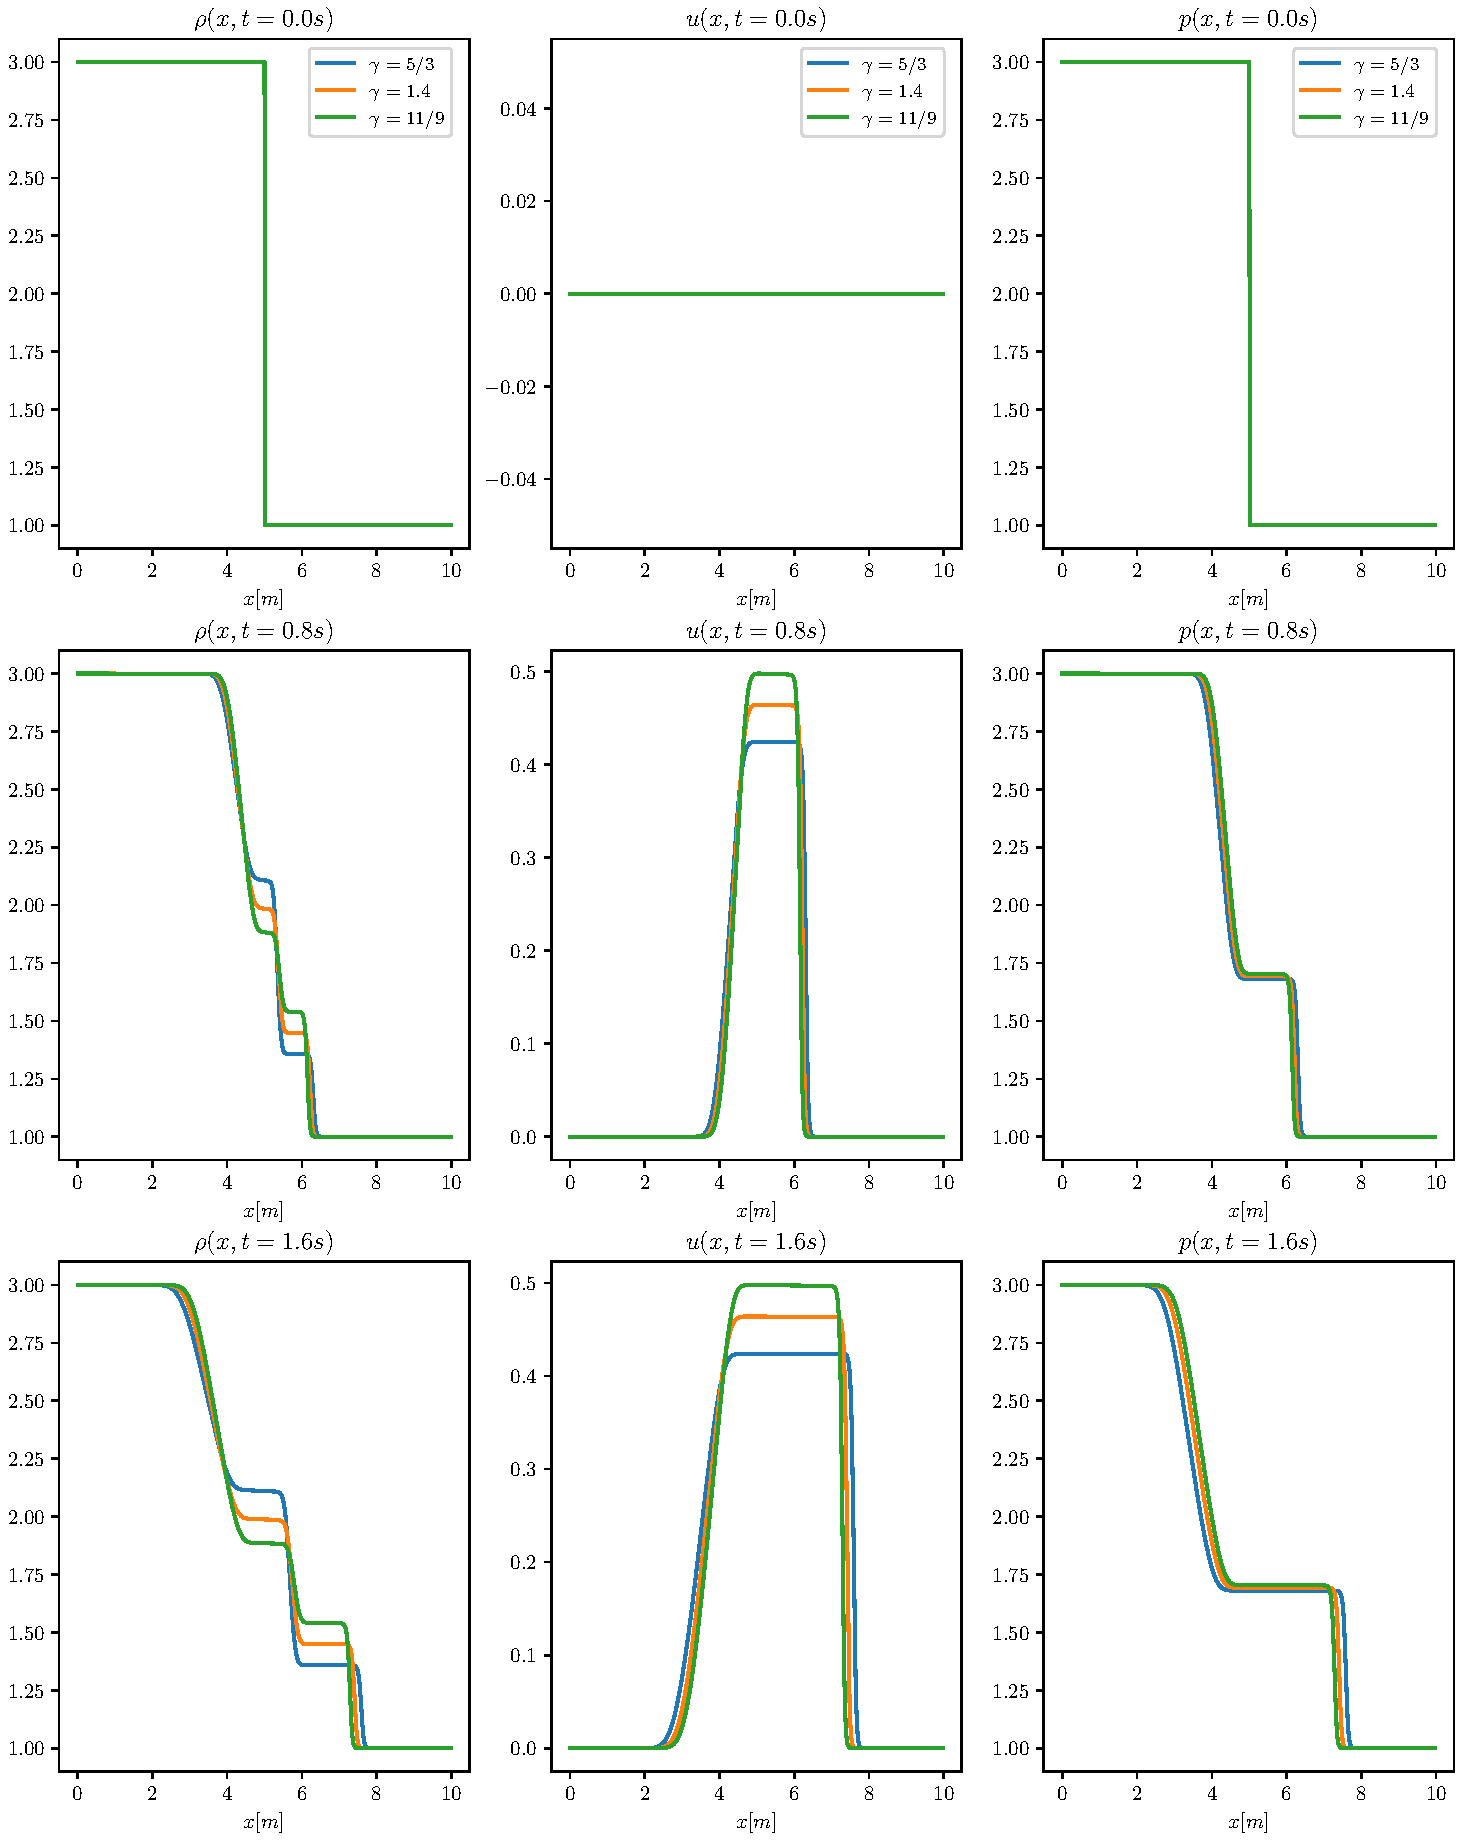
\includegraphics[width=\linewidth]{../euler1D/experimentos/graficas_sod/1.pdf}
	\caption{Primeros tres instantes de las simulaciones con distintos $\gamma$.}
\end{figure}
\begin{figure}[H]
	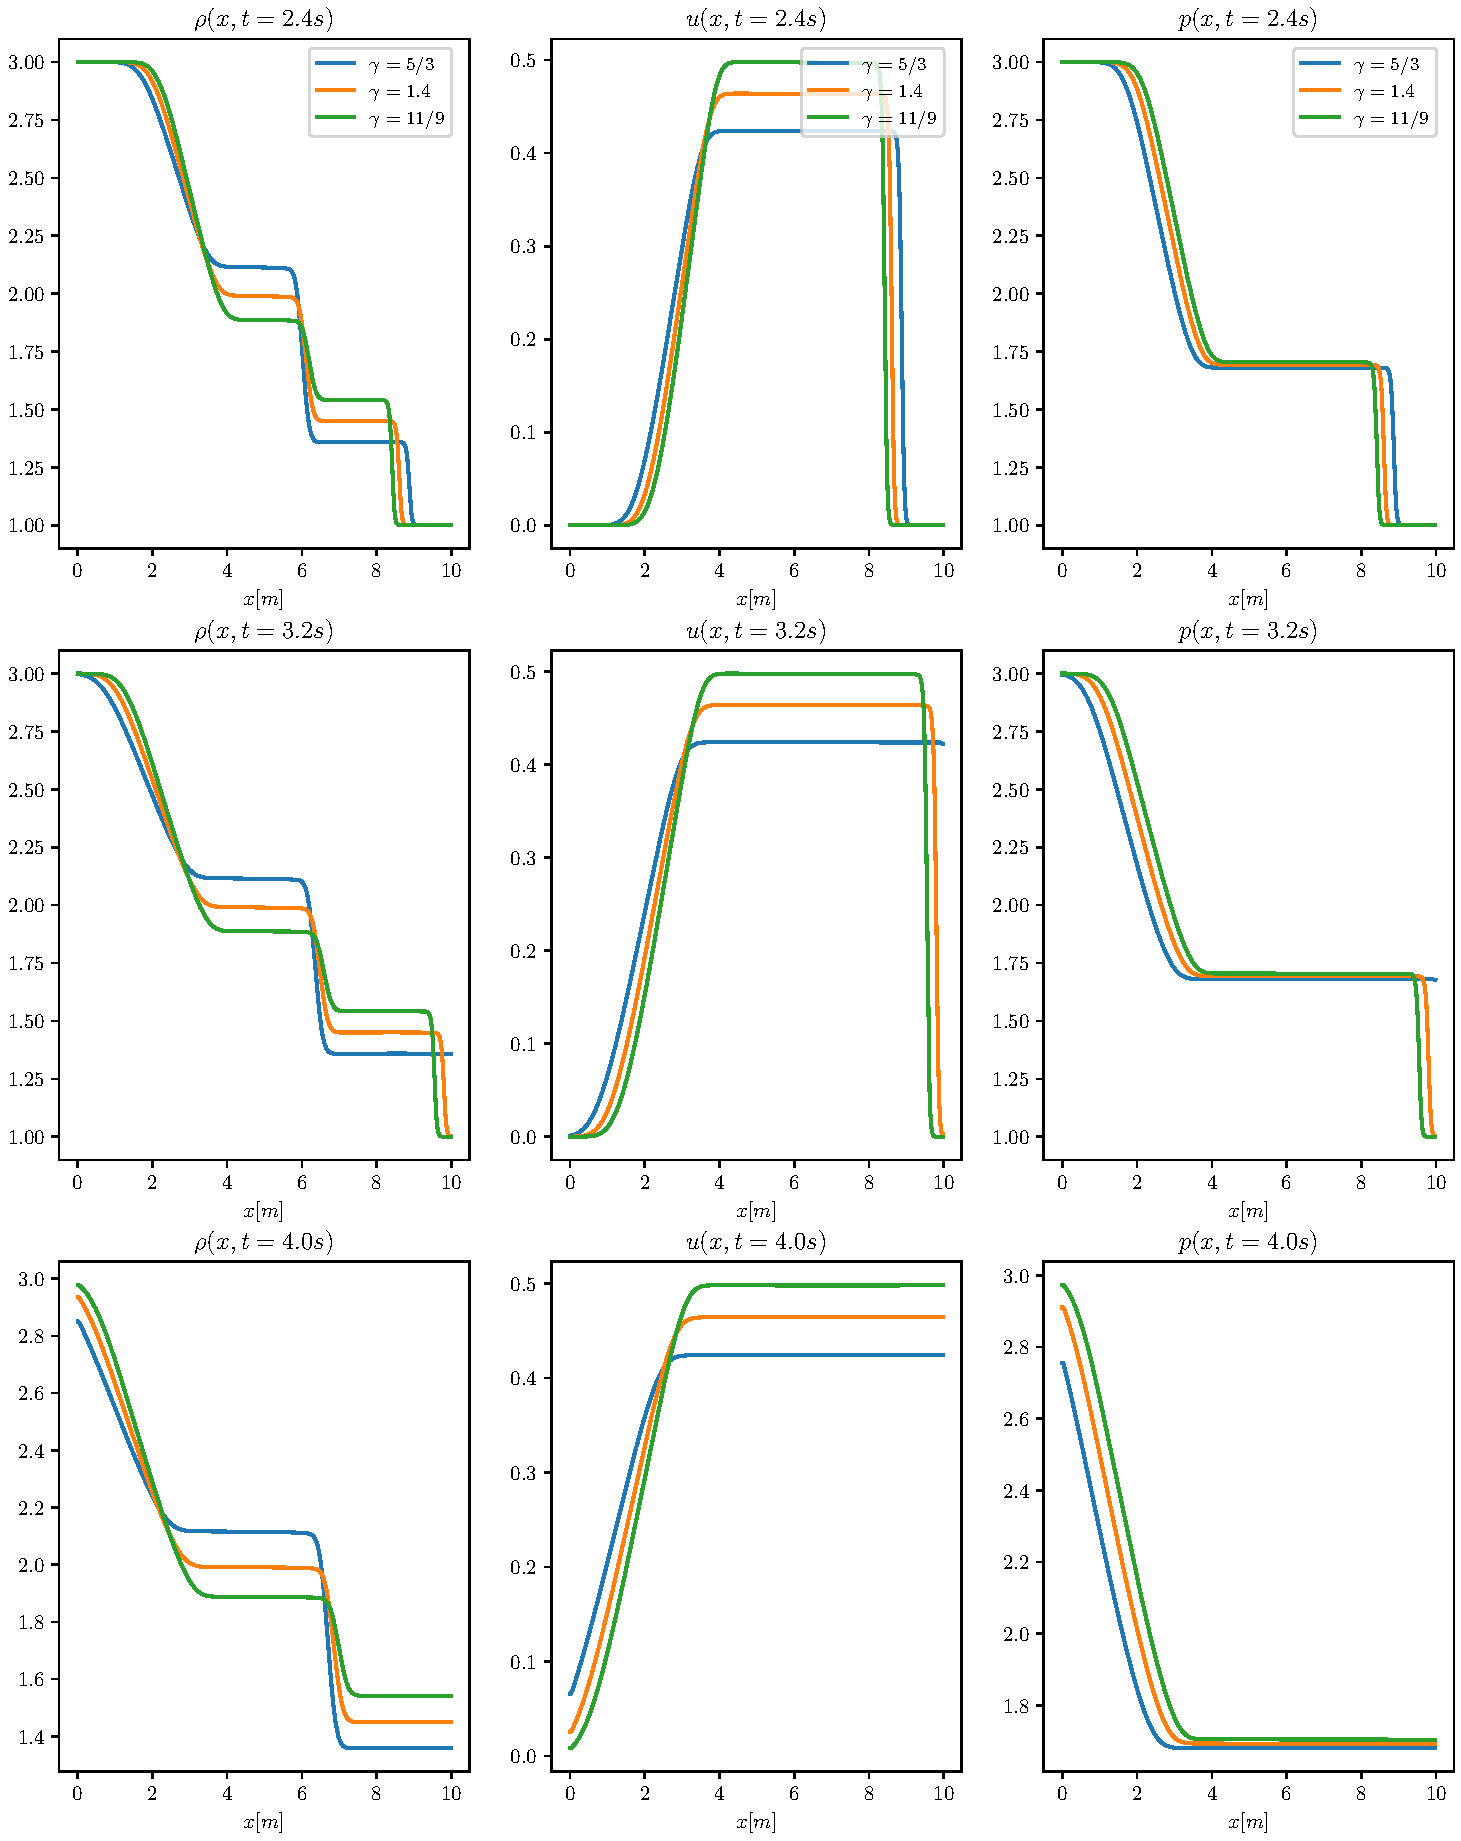
\includegraphics[width=\linewidth]{../euler1D/experimentos/graficas_sod/2.pdf}
	\caption{Últimos tres instantes de las simulaciones con distintos $\gamma$.}
\end{figure}

\subsection{Observaciones}